\section{Data and Benchmark}
\label{sec:data}
% System architecture figure (hand-drawn TikZ; included from sections/method.tex).
% Source of truth for the shapes: src/translit/models.py (TransformerS2S), noise.py (OPS),
% augment.py (conditions A0-A4, CTRL), decode.py (beam_search), finetune.py (v2 deployment model).
\begin{figure*}[t]
\centering
\resizebox{\textwidth}{!}{%
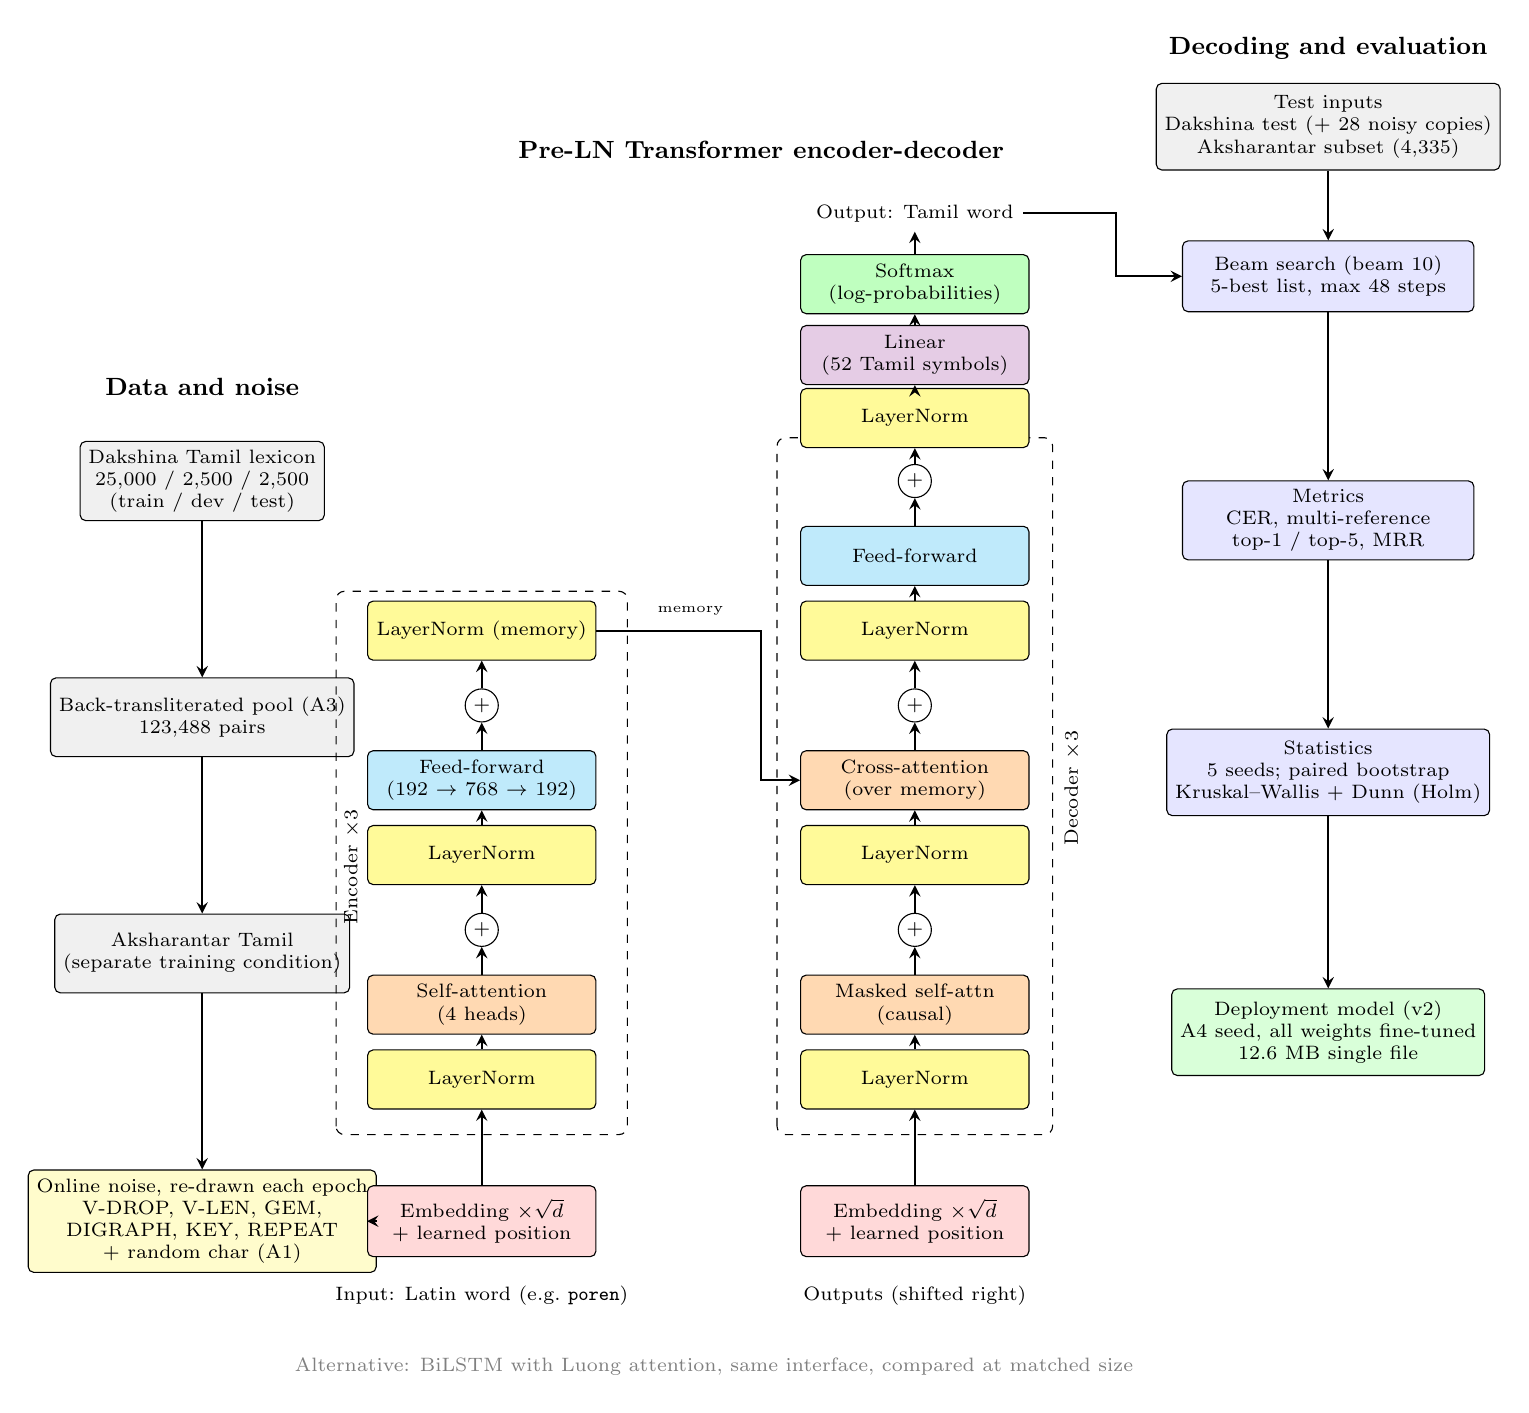
\begin{tikzpicture}[
  blk/.style={draw, rounded corners=2pt, minimum width=2.9cm, minimum height=0.75cm, font=\scriptsize, align=center, inner sep=3pt},
  emb/.style={blk, fill=red!15, minimum height=0.9cm},
  att/.style={blk, fill=orange!30},
  ffn/.style={blk, fill=cyan!25},
  nrm/.style={blk, fill=yellow!40},
  outp/.style={blk, fill=violet!20},
  smx/.style={blk, fill=green!25},
  dat/.style={blk, minimum width=3.0cm, fill=gray!12, minimum height=1.0cm},
  add/.style={circle, draw, inner sep=0pt, minimum size=0.42cm, font=\scriptsize},
  grp/.style={draw, dashed, rounded corners=3pt},
  arr/.style={->, >=stealth, thick},
]

% ---------- Column A: data and noise ----------
\node[font=\small\bfseries] at (1.5,11.6) {Data and noise};
\node[dat] (a1) at (1.5,10.4) {Dakshina Tamil lexicon\\25{,}000 / 2{,}500 / 2{,}500\\(train / dev / test)};
\node[dat] (a2) at (1.5,7.4) {Back-transliterated pool (A3)\\123{,}488 pairs};
\node[dat] (a3) at (1.5,4.4) {Aksharantar Tamil\\(separate training condition)};
\node[dat, minimum height=1.3cm, fill=yellow!20] (a4) at (1.5,1.0) {Online noise, re-drawn each epoch\\V-DROP, V-LEN, GEM,\\DIGRAPH, KEY, REPEAT\\+ random char (A1)};
\draw[arr] (a1) -- (a2);
\draw[arr] (a2) -- (a3);
\draw[arr] (a3) -- (a4);

% ---------- Column B: Transformer encoder-decoder ----------
\node[font=\small\bfseries] at (8.6,14.6) {Pre-LN Transformer encoder-decoder};

% Encoder (source = romanized word)
\node[emb] (e1) at (5.05,1.0) {Embedding $\times\sqrt{d}$\\+ learned position};
\node[nrm] (e2) at (5.05,2.8) {LayerNorm};
\node[att] (e3) at (5.05,3.75) {Self-attention\\(4 heads)};
\node[add] (e4) at (5.05,4.7) {$+$};
\node[nrm] (e5) at (5.05,5.65) {LayerNorm};
\node[ffn] (e6) at (5.05,6.6) {Feed-forward\\(192 $\rightarrow$ 768 $\rightarrow$ 192)};
\node[add] (e7) at (5.05,7.55) {$+$};
\node[nrm] (en) at (5.05,8.5) {LayerNorm (memory)};
\draw[grp] (3.2,2.1) rectangle (6.9,9.0);
\node[rotate=90, font=\scriptsize] at (3.4,5.5) {Encoder $\times 3$};
\draw[arr] (e1) -- (e2);
\draw[arr] (e2) -- (e3);
\draw[arr] (e3) -- (e4);
\draw[arr] (e4) -- (e5);
\draw[arr] (e5) -- (e6);
\draw[arr] (e6) -- (e7);
\draw[arr] (e7) -- (en);

% Decoder (target shifted right, causal)
\node[emb] (d1) at (10.55,1.0) {Embedding $\times\sqrt{d}$\\+ learned position};
\node[nrm] (d2) at (10.55,2.8) {LayerNorm};
\node[att] (d3) at (10.55,3.75) {Masked self-attn\\(causal)};
\node[add] (d4) at (10.55,4.7) {$+$};
\node[nrm] (d4n) at (10.55,5.65) {LayerNorm};
\node[att] (d5) at (10.55,6.6) {Cross-attention\\(over memory)};
\node[add] (d6) at (10.55,7.55) {$+$};
\node[nrm] (d7) at (10.55,8.5) {LayerNorm};
\node[ffn] (d8) at (10.55,9.45) {Feed-forward};
\node[add] (d9) at (10.55,10.4) {$+$};
\draw[grp] (8.8,2.1) rectangle (12.3,10.95);
\node[rotate=90, font=\scriptsize] at (12.55,6.5) {Decoder $\times 3$};
\draw[arr] (d1) -- (d2);
\draw[arr] (d2) -- (d3);
\draw[arr] (d3) -- (d4);
\draw[arr] (d4) -- (d4n);
\draw[arr] (d4n) -- (d5);
\draw[arr] (d5) -- (d6);
\draw[arr] (d6) -- (d7);
\draw[arr] (d7) -- (d8);
\draw[arr] (d8) -- (d9);

% Memory from encoder into decoder cross-attention
\draw[arr] (en.east) -- (8.6,8.5) |- (d5.west);
\node[font=\tiny] at (7.7,8.75) {memory};

% Output head
\node[nrm] (of) at (10.55,11.2) {LayerNorm};
\node[outp] (o1) at (10.55,12.0) {Linear\\(52 Tamil symbols)};
\node[smx] (o2) at (10.55,12.9) {Softmax\\(log-probabilities)};
\node[font=\scriptsize] (o3) at (10.55,13.8) {Output: Tamil word};
\draw[arr] (d9) -- (of);
\draw[arr] (of) -- (o1);
\draw[arr] (o1) -- (o2);
\draw[arr] (o2) -- (o3);

% Inputs
\node[font=\scriptsize] at (5.05,0.05) {Input: Latin word (e.g.\ \texttt{poren})};
\node[font=\scriptsize] at (10.55,0.05) {Outputs (shifted right)};
\draw[arr] (a4.east) -- (e1.west);
\node[font=\scriptsize, text=gray] at (8.0,-0.85) {Alternative: BiLSTM with Luong attention, same interface, compared at matched size};

% ---------- Column C: decoding and evaluation ----------
\node[font=\small\bfseries] at (15.8,15.9) {Decoding and evaluation};
\node[dat, minimum height=1.1cm] (t0) at (15.8,14.9) {Test inputs\\Dakshina test (+ 28 noisy copies)\\Aksharantar subset (4{,}335)};
\node[blk, fill=blue!10, minimum width=3.7cm, minimum height=0.9cm] (c1) at (15.8,13.0) {Beam search (beam 10)\\5-best list, max 48 steps};
\node[blk, fill=blue!10, minimum width=3.7cm, minimum height=1.0cm] (c2) at (15.8,9.9) {Metrics\\CER, multi-reference\\top-1 / top-5, MRR};
\node[blk, fill=blue!10, minimum width=3.7cm, minimum height=1.1cm] (c3) at (15.8,6.7) {Statistics\\5 seeds; paired bootstrap\\Kruskal--Wallis + Dunn (Holm)};
\node[blk, fill=green!15, minimum width=3.7cm, minimum height=1.1cm] (c4) at (15.8,3.4) {Deployment model (v2)\\A4 seed, all weights fine-tuned\\12.6 MB single file};
\draw[arr] (t0) -- (c1);
\draw[arr] (c1) -- (c2);
\draw[arr] (c2) -- (c3);
\draw[arr] (c3) -- (c4);
\draw[arr] (o3.east) -- (13.1,13.8) |- (c1.west);

\end{tikzpicture}%
}
\caption{Architecture of the system. Left: the data sources, and the noise that is re-drawn online each epoch (six Tamil-specific operators, plus random character noise for A1). Centre: the pre-LN Transformer encoder-decoder used in the main comparison (three layers per side, four heads, $d{=}192$, feed-forward width 768, learned positions; 3.15M parameters at the deployment size). Each sublayer is LayerNorm, then the sublayer, then the residual addition ($+$); the encoder output passes through a final LayerNorm to the decoder's cross-attention. Right: test inputs are decoded with beam search (beam 10) and scored; statistics use five seeds and paired bootstrap; the best A4 seed is fine-tuned into the deployment model.}
\label{fig:architecture}
\end{figure*}

\textbf{Training and clean evaluation.}
We use the Dakshina Tamil romanization lexicon: 25{,}000 training words (68{,}218 romanization pairs), 2{,}500 development words (6{,}827 pairs) and 2{,}500 test words (6{,}864 pairs), which are word-disjoint~\cite{roark2020dakshina}.
Inputs are lowercase Latin and outputs are NFC-normalised Tamil.
A romanization attested for several native forms is scored against all of them.
The development set is used only for early stopping and tuning.
The test lexicon holds 6{,}833 distinct romanized inputs.

\textbf{Independent test sets.}
Aksharantar's Tamil test file contains every Dakshina test pair~\cite{madhani2023aksharantar}.
We keep only rows whose native word occurs in no Dakshina split, which gives three subsets by source: AK-Freq (2{,}607 distinct inputs, frequent web words), AK-NEI (991) and AK-NEF (706), plus their union AK-all.
We also found that Aksharantar's training file shares stems with Dakshina test words, so we never train on it in the controlled experiments.

\textbf{Paired noisy test sets.}
Seven operators perturb the romanized input only (\Cref{tab:ops}).
Each of the 6{,}833 test inputs is perturbed at severity $p\in\{0.1,0.2,0.3,0.5\}$ with a random seed derived from the word, operator and severity.
The 28 sets are therefore exactly reproducible, and each noisy item stays paired with its clean form and references.
Operators and rates are motivated by the typing phenomena in the literature~\cite{wolfsonkin2019latin,herath2024tamzhi,belinkov2018synthetic}.
The digraph operator swaps in both directions (th$\leftrightarrow$t, dh$\leftrightarrow$d, sh$\leftrightarrow$s, ch$\leftrightarrow$c,s) and maps zh to l or z only one way, because in our own measurement on public code-mixed Tamil comments~\cite{chakravarthi2020tamilmix} (heuristic, unverified by hand) vowel dropping, vowel-length collapse and stretching occur several times more often than in Dakshina, while dropped h does not.
\Cref{tab:ops} reports realised strength: nominal $p$ is a per-position probability, so we report the share of words changed; the character edit rate at $p{=}0.3$ is 12.7\% for V-DROP, 7.4\% for KEY and 15.8\% for MIX (see the repository manifest for all sets).

\begin{table}[t]
\caption{Noise operators and the share of test words they change (\%) at three severities.}
\label{tab:ops}
\centering\footnotesize
\resizebox{\columnwidth}{!}{\begin{tabular}{llccc}
\toprule
Operator & Effect & \multicolumn{3}{c}{Words changed (\%) at $p=$} \\
\cmidrule(lr){3-5}
 & & 0.1 & 0.3 & 0.5 \\
\midrule
V-DROP & delete non-initial vowels & 34 & 73 & 89 \\
V-LEN & collapse doubled vowels & 4 & 13 & 21 \\
GEM & collapse doubled consonants & 3 & 9 & 15 \\
DIGRAPH & th/t, dh/d, sh/s, ch/c/s swaps; zh$\to$l,z & 12 & 32 & 47 \\
KEY & adjacent QWERTY key substitution & 21 & 52 & 69 \\
REPEAT & stretch one vowel by 1--3 letters & 10 & 29 & 51 \\
MIX & random combination of the six & 35 & 69 & 82 \\
\bottomrule
\end{tabular}}
\end{table}

\textbf{Synthetic training data.}
For the augmentation study we construct a pool of 60{,}000 further Tamil words from the IndicXlit unigram list.
We remove every Dakshina word, every independent-test word and any word sharing a five-code-point prefix with a held-out word (46{,}652 of 137{,}748 candidates were removed for stem overlap alone).
A Tamil-to-Latin BiLSTM trained on Dakshina romanizes each pool word three times by sampling at temperature 1; a closeness filter against the model's greedy output drops 17{,}828 degenerate samples and leaves 123{,}488 pairs.
A control set romanizes the same 60{,}000 words once, greedily (60{,}000 pairs).
These romanizations are machine-made, so they carry the errors of the model that made them.
